\documentclass[12pt, a4paper]{report}

% ==================== PACKAGES ====================
\usepackage[utf8]{inputenc}
\usepackage{graphicx}       % For handling images and logos
\usepackage{geometry}       % For page margins
\usepackage{setspace}       % For line spacing (1.5 spacing)
\usepackage{times}          % Times New Roman font
\usepackage{titlesec}       % To customize chapter titles
\usepackage{tocloft}        % To customize Table of Contents
\usepackage{array}          % For better table formatting
\usepackage{hyperref}       % For clickable links in PDF
\hypersetup{
    pdfborder={0 0 0}
}
\usepackage{fancyhdr}       % For headers and footers
\usepackage{caption}        % For caption formatting
\usepackage{indentfirst}
\usepackage{tikz}
\usetikzlibrary{calc, shapes.geometric, arrows, positioning}


% ==================== PAGE SETUP ====================
% Standard thesis margins: Left 1.5in (for binding), others 1in
\geometry{left=1.5in, right=1.0in, top=0.8in, bottom=0.8in}

% 1.5 Line Spacing
\onehalfspacing

% Center Chapter Headings and reduce top margin for chapters
\titleformat{\chapter}[display]
  {\normalfont\huge\bfseries\centering}
  {\chaptertitlename\ \thechapter}{20pt}{\Huge}
\titlespacing*{\chapter}{0pt}{-30pt}{20pt}

% ==================== DOCUMENT DETAILS ====================
\newcommand{\projectTitle}{Virtual Try-On: An AI-Powered Local Virtual Try-On Studio with VRAM-Optimized Hybrid Pipelines}
\newcommand{\studentOne}{Geethesh H S (1BY25SCS02)}
\newcommand{\studentTwo}{}
% \newcommand{\studentThree}{Student Name 3 (USN)}
% \newcommand{\studentFour}{Student Name 4 (USN)}
\newcommand{\guideName}{Dr. Raguru Jaya Krishna }
\newcommand{\guideDesignation}{Associate Professor}
\newcommand{\clusterHeadName}{Dr. Shoba M}
\newcommand{\clusterHeadDesignation}{Associate Professor}
\newcommand{\hodName}{Dr. Satish Kumar T}
\newcommand{\principalName}{Dr. Sanjay H A}
\newcommand{\deptName}{Department of Computer Science and Engineering}
\newcommand{\collegeName}{BMS INSTITUTE OF TECHNOLOGY AND MANAGEMENT}
\newcommand{\collegeAddressA}{(Autonomous Institute under VTU, Belagavi, Karnataka - 590 018)}
\newcommand{\collegeAddressB}{Yelahanka, Bengaluru, Karnataka - 560119}
\newcommand{\academicYear}{2025-26}

% ==================== BEGIN DOCUMENT ====================
\begin{document}

% --------------------------------------------------------
% 1. COVER PAGE 
% --------------------------------------------------------
\begin{titlepage}

% --- START OF BORDER CODE ---
    \begin{tikzpicture}[remember picture, overlay]
        \draw[line width=1.5pt] % Adjust thickness here (e.g., 2pt, 3pt)
        ($(current page.north west) + (1.5cm,-1.5cm)$) % Top-left margin
        rectangle
        ($(current page.south east) + (-1.5cm,1.5cm)$); % Bottom-right margin
    \end{tikzpicture}
    % --- END OF BORDER CODE ---
    
    \begin{center}
        \textbf{\large VISVESVARAYA TECHNOLOGICAL UNIVERSITY}\\[0.2cm]
        \textbf{\small Jnana Sangama, Belagavi, Karnataka - 590018}\\[0.5cm]
        
        % COLLEGE LOGO
        \includegraphics[width=3.5cm]{vtu_logo.png} \\[0.5cm]
        \textbf{\large Machine Learning (25MCS21) 
 }\\[0.3cm]

        \textbf{\large "CCA Report on"}\\[0.3cm]
        \textbf{\Large \projectTitle}\\[0.5cm]
        
        \textit{Submitted in partial fulfilment of the requirements for the conferment of degree of}\\[0.3cm]
        \textbf{\large MASTER OF TECHNOLOGY}\\[0.2cm]
        \textit{in}\\[0.2cm]
        \textbf{\large COMPUTER SCIENCE AND ENGINEERING}\\[0.5cm]
        
        \textit{by}\\[0.3cm]
        \textbf{\studentOne}\\[0.5cm]
        
        \textit{Under the Guidance of}\\[0.2cm]
        \textbf{\guideName}\\
        \textit{\guideDesignation}\\[0.5cm]
        
        \textbf{\deptName}\\[0.3cm]
        
        % COLLEGE LOGO
        \includegraphics[width=3.5cm]{bmsit_logo.png} \\[0.3cm]
        
        \textbf{\large \collegeName}\\
        \small \collegeAddressA\\
        \small \collegeAddressB
        
    \end{center}
\end{titlepage}


% --------------------------------------------------------
% 4. ACKNOWLEDGEMENT 
% --------------------------------------------------------
\newpage
\chapter*{ACKNOWLEDGEMENT}
\thispagestyle{empty}
\addcontentsline{toc}{chapter}{Acknowledgement}

\indent I would like to express my heartfelt gratitude to everyone who has contributed to make this project a memorable experience and has inspired this work in some way.

Let me begin by expressing my gratitude to the Almighty God for the numerous blessings bestowed upon me. We are happy to present this project after completing it successfully.

This project would not have been possible without the guidance, assistance, and suggestions of many individuals. We express our deep sense of gratitude and indebtedness to each and every one who has helped us make this project a success.

We heartily thank \textbf{\principalName}, Principal, BMS Institute of Technology \& Management for constant encouragement and inspiration in taking up this project.

We heartily thank \textbf{\hodName}, HoD, Department of Computer Science and Engineering, BMS Institute of Technology \& Management for constant encouragement and inspiration in taking up this project.

We heartily thank \textbf{\clusterHeadName}, Division-2 Head, BMS Institute of Technology \& Management for constant encouragement and inspiration in taking up this project.

We gratefully thank our project guide, \textbf{\guideName}, for guidance and support throughout the course of the project work.

Special thanks to all the staff members of the Computer Science and Engineering Department for their help and kind co-operation. Lastly, we thank our parents and friends for their encouragement and support in helping us complete this work.

\vspace{1cm}
\begin{flushright}
\textbf{\studentOne}
\end{flushright}

% --------------------------------------------------------
% 5. DECLARATION 
% --------------------------------------------------------
\newpage
\chapter*{DECLARATION}
\addcontentsline{toc}{chapter}{Declaration}

We, hereby declare that the project titled \textbf{``\projectTitle''} is a record of original project work under the guidance of \textbf{\guideName, \guideDesignation}, Department of Computer Science and Engineering, BMS Institute of Technology \& Management, Autonomous Institute under Visvesvaraya Technological University, Belagavi during the Academic Year \academicYear.

I also declare that this project report has not been submitted for the award of any degree, diploma, associateship, fellowship or other title anywhere else.

\vspace{1cm}
\begin{table}[h]
\centering
\begin{tabular}{|c|c|c|}
\hline
\textbf{Name of the Student} & \textbf{USN} & \textbf{   Signature   } \\ \hline
\rule{0pt}{3ex} Geethesh H S & 1BY25SCS02 &  \\ \hline
\end{tabular}
\end{table}

% --------------------------------------------------------
% 6. ABSTRACT 
% --------------------------------------------------------
\chapter*{ABSTRACT}
\addcontentsline{toc}{chapter}{Abstract}
Rapid advancements in generative artificial intelligence and deep neural networks have fundamentally transformed the digital fashion domain, introducing novel mechanisms for virtual try-on systems. The virtual try on is a production-quality, 100\% local, AI-powered Virtual Try-On (VTON) web application engineered to operate on resource-constrained consumer GPUs. The framework combines a highly responsive, modern React frontend built with Vite and Tailwind CSS and an asynchronous FastAPI backend utilizing PyTorch and Hugging Face Diffusers to perform virtual garment dressing and text-guided clothing modifications locally, ensuring absolute user data privacy and removing reliance on subscription-based cloud APIs.

To execute realistic virtual dressing, the framework integrates three specialized deep learning modules. First, a semantic clothing segmentation service powered by a localized SegFormer architecture parses the subject image to isolate specific clothing boundaries and generate a soft binary mask using OpenCV morphological dilation. Second, a direct virtual try-on module utilizes the CatVTON (``Concatenation Is All You Need'') architecture, which uses spatial concatenation of latents in a custom diffusers pipeline to transfer garment textures onto the masked region. Third, a text-guided wardrobe editor automatically switches to a Stable Diffusion 1.5 Inpainting pipeline to apply modifications specified via natural language instructions, enabling interactive and flexible wardrobe personalization.

A major technical achievement of the virtual try on is its suite of hardware-aware optimizations designed to operate within a 4GB Video RAM (VRAM) threshold, common on NVIDIA RTX 3050 Laptop GPUs. By implementing a custom model manager for active device offloading, executing half-precision (FP16) CUDA computations, and enabling tiled and sliced Variational Autoencoder (VAE) latent processing, the system comfortably runs complex diffusion pipelines without Out-of-Memory (OOM) failures. Experimental evaluations demonstrate the efficacy of the proposed system in rendering realistic high-fidelity outputs with low inference latency, providing a robust, private, and accessible solution for local virtual try-on applications.

% --------------------------------------------------------
% 7. TABLE OF CONTENTS 
% --------------------------------------------------------
\newpage
\tableofcontents


% --------------------------------------------------------
% 8. LIST OF FIGURES & TABLES 
% --------------------------------------------------------



% Use Arabic numerals for chapter pages

% --------------------------------------------------------
% CHAPTER 1: INTRODUCTION 
% --------------------------------------------------------
\chapter{Introduction}

\section{Overview}

In recent years, the intersection of computer vision, deep learning, and digital commerce has accelerated the adoption of immersive virtual experiences. Among these, Virtual Try-On (VTON) technologies have emerged as a key application, allowing users to visualize how garments would look on them without visiting physical dressing rooms. The ability to realistically adapt clothing items to varying body shapes, folds, poses, and lighting conditions remains a core research frontier in generative computer vision.

The virtual try on is a production-quality, 100\% local, AI-powered Virtual Try-On studio designed to run on consumer hardware. The framework provides a dual-inference mechanism: direct virtual try-on utilizing a spatial-concatenation attention model (CatVTON) and text-guided clothing edits using a Stable Diffusion 1.5 Inpainting pipeline. By processing inputs directly on the user's machine, the virtual try on avoids the privacy concerns, high operating costs, and latency issues associated with remote, cloud-based generative AI APIs.

\section{Problem Statement}

Existing virtual try-on systems suffer from several limitations that restrict their widespread application. Commercial VTON services are almost exclusively hosted in the cloud, requiring users to upload sensitive personal photographs to external servers, creating significant data privacy and security risks. Additionally, cloud services operate on subscription-based models or API-call fee structures, which can compile prohibitive costs for scaling businesses and developers.

From a technical standpoint, open-source local try-on implementations are often heavy and suffer from extreme memory footprints, demanding high-end enterprise GPUs with 8GB to 24GB of Video RAM (VRAM) to perform inference. When deployed on consumer-grade hardware (such as laptops equipped with NVIDIA RTX 3050 GPUs featuring 4GB VRAM), these models trigger Out-of-Memory (OOM) crashes. Furthermore, conventional systems lack a unified pipeline that can seamlessly transition between direct texture wrapping (dressing the user in a specific uploaded garment) and text-guided semantic editing (such as changing the fabric type, color, or design of a shirt using natural language prompts).

\section{Motivation}

The core motivation behind the virtual try on is to democratize high-fidelity virtual dressing technology by making it highly optimized, local, private, and accessible on affordable hardware. Enabling complex generative diffusion models to execute locally on 4GB VRAM laptops allows developers and small businesses to utilize advanced try-on capabilities without capital expenditures on cloud infrastructure.

Furthermore, the rapid progress of latent diffusion models and transformer-based semantic segmentations provides an opportunity to build a unified system. Integrating SegFormer for automatic mask generation, CatVTON for pose-insensitive garment mapping, and Stable Diffusion for language-guided edits into a single local studio workflow enables a comprehensive e-commerce prototyping tool. This design removes the need for physical apparel samples or expensive photo shoots, accelerating creative iteration.

\section{Scope of the Project}

The scope of the virtual try on comprises the development of an optimized local virtual try-on application featuring:

\begin{itemize}
\item A modular, responsive React frontend client built with Vite and styled with Tailwind CSS, offering drag-and-drop file upload, webcam capture, and split-pane before-after visualization.
\item An asynchronous FastAPI backend server implementing multi-stage image pre-processing, aspect-ratio scaling, and dynamic cleanup tasks to prevent disk leakage.
\item An automated segmentation module using a localized SegFormer architecture to generate clothing-agnostic masks with OpenCV boundary feathering.
\item An AI inference engine supporting direct VTON (CatVTON) and prompt-based clothing inpainting (Stable Diffusion 1.5).
\item A hardware-aware model manager executing active device weight offloading, FP16 half-precision execution, and VAE latent tiling and slicing to support execution under the 4GB VRAM ceiling.
\end{itemize}

The project is structured to run offline, ensuring zero external API dependencies and robust performance on desktop or laptop environments equipped with CUDA-capable GPUs.

% --------------------------------------------------------
% CHAPTER 2: LITERATURE REVIEW
% --------------------------------------------------------
\chapter{Literature Review}

\section{Introduction}

The development of image-based virtual try-on systems has progressed through multiple paradigm shifts. Early attempts relied on 3D computer graphics and physical simulations to drape digital garments over reconstructed 3D body models. Although structurally consistent, these systems were computationally heavy, required complex manual setup, and lacked visual realism. The focus subsequently shifted toward deep learning methods, which utilize large image datasets to learn realistic mapping and textures directly in the pixel domain.

This chapter analyzes the evolution of deep learning approaches for virtual try-on, evaluating Generative Adversarial Networks (GANs), Diffusion Models, Attention-based warping frameworks, Semantic Segmentation, and the hardware optimizations required to run these architectures.

\section{Generative Adversarial Network Based Approaches}

Generative Adversarial Networks (GANs) established the initial standard for deep-learning-based virtual try-on. Frameworks such as VITON and CP-VTON introduced a two-stage approach: first, warping the clothing image to match the body pose, and second, generating a composite image using an adversarial generator. Warping was typically achieved using Thin-Plate Spline (TPS) algorithms or optical flow estimation.

Warping networks, however, frequently fail to handle complex poses, occlusion boundaries, and high-frequency details (such as text logo prints or intricate folds). If the initial geometric warp is incorrect, the final generated image displays distortion. Additionally, GAN-based systems suffer from training instability, mode collapse, and a lack of semantic flexibility, meaning they cannot perform edits using textual descriptions.

\section{Diffusion-Based Virtual Try-on}

Denoising Diffusion Probabilistic Models (DDPMs) and Latent Diffusion Models (LDMs) have revolutionized image synthesis, providing superior visual fidelity and diversity compared to GANs. By formulating generation as an iterative denoising process, diffusion models reconstruct highly realistic fabric folds, shadows, and body-clothing boundaries.

Inpainting pipelines, such as Stable Diffusion Inpainting, leverage conditioning signals (such as text prompts and binary masks) to edit specific portions of an image while preserving the unmasked pixels. While diffusion models demonstrate robust synthesis, adapting them for direct virtual try-on requires mapping the exact texture of a reference garment onto a target mask. This process can be challenging because standard text-to-image models lack fine-grained structural constraints, which can lead to alterations in garment patterns, logos, or brand identities.

\section{Spatial Concatenation and Attention Mechanisms}

To solve the limitations of geometric warping and text-to-image mismatch, recent architectures focus on alignment-free try-on pipelines. The CatVTON (``Concatenation Is All You Need'') model implements this concept by bypassing explicit warping modules entirely.

Instead of warping the garment in 2D space prior to generation, CatVTON performs spatial concatenation of the person image, clothing-agnostic mask, and garment image directly in the latent space. By passing the concatenated representation through a shared U-Net structure, the model leverages skip-cross-attention layers to correlate feature tokens between the garment and the target body mask. This attention-driven transfer preserves complex textures, patterns, and logos, maintaining high structural fidelity.

\section{Segment-Based Clothing Extraction}

Generating the binary mask that represents the region of the clothing to be replaced is a critical step in virtual try-on. Manual mask generation is inefficient and impractical for real-time applications. To address this, semantic segmentation models are utilized to parse body parts and apparel.

SegFormer, an efficient transformer-based semantic segmentation framework, integrates hierarchical ViT encoders with lightweight MLP decoders. By training SegFormer on clothing datasets (such as the `segformer\_b2\_clothes` checkpoint), it extracts pixel-level classifications for various garments (e.g., upper-clothes, pants, skirts, and dresses). Applying morphological dilation using OpenCV to the segmented outputs generates clothing-agnostic masks that can blend with the generated textures at the boundaries.

\section{Research Gap}

Despite the capabilities of modern models like CatVTON and Stable Diffusion, a gap exists in software deployment. Most research repositories focus on isolated, offline scripts that run on high-VRAM enterprise servers, ignoring the constraints of standard consumer GPUs.

Furthermore, existing solutions do not provide an integrated, local application that combines:
\begin{enumerate}
\item Automated clothes parsing using SegFormer segmentation.
\item Spatial-concatenation direct try-on using CatVTON.
\item Semantic text-guided modifications using Stable Diffusion Inpainting.
\end{enumerate}
There is a need for a unified web framework that manages VRAM consumption on consumer hardware, enabling seamless execution on laptop GPUs with 4GB VRAM.

\section{Proposed Contribution}

The virtual try on addresses these limitations by introducing a local, optimized virtual try-on studio. The framework provides a hybrid pipeline that handles both direct try-on (for texture transfer) and prompt-guided editing (for semantic modifications).

The main technical contributions of the virtual try on include:
\begin{itemize}
\item An automatic mask generator that extracts, dilates, and feathers clothing masks using SegFormer and OpenCV.
\item A dynamic Model Manager that offloads inactive model weights (e.g., swapping CatVTON and SD Inpaint pipelines between CUDA and CPU) to manage VRAM usage.
\item VRAM optimization techniques (half-precision FP16, VAE slicing, and tiling) to enable execution under a 4GB memory ceiling.
\item An asynchronous FastAPI server paired with a React frontend client to provide an interactive development environment.
\end{itemize}

%--------------------------------------------
% CHAPTER 3: SYSTEM DESIGN AND METHODOLOGY
% --------------------------------------------------------
\chapter{System Design and Methodology}

\section{Introduction}

The development of the virtual try on requires a system architecture that handles multi-stage image processing, semantic segmentation, latent space diffusion, and memory optimization. The system is designed to provide an interactive workspace where users can upload images, perform automatic masking, and generate try-on results with low latency. This chapter details the system architecture, component modules, mathematical formulations, and operational workflow of the framework.

\text{System Architecture}

The system follows a client-server model, separating frontend visualization from backend inference. The backend coordinates the SegFormer segmentation model, the CatVTON model, and the Stable Diffusion Inpaint model through a centralized `ModelManager`.

The overall workflow of the system is illustrated below:

\begin{center}
User Upload (Person \& Garment Images)

$\downarrow$

FastAPI Upload Handlers

$\downarrow$

SegFormer Clothing Segmentation

$\downarrow$

OpenCV Morphological Dilation \& Gaussian Feathering (Agnostic Mask)

$\downarrow$

Pipeline Decision (Is Text Prompt Empty?)

$\swarrow \quad\quad\quad\quad\quad\quad \searrow$

[Yes] Direct Try-On (CatVTON)  \quad\quad\quad\quad [No] Text-guided Edits (SD Inpaint)

$\searrow \quad\quad\quad\quad\quad\quad \swarrow$

Mask-based Repainting / Blending (Pillow)

$\downarrow$

Vite Frontend (Rendered Result via Before-After Slider)
\end{center}

\section{Input Acquisition and Processing Module}

The input acquisition module handles two primary image assets: the target person image ($I_{person}$) and the reference garment image ($I_{cloth}$). The React frontend client allows users to upload these images via drag-and-drop interfaces or capture the target person image in real time using a webcam interface.

Upon receiving the files, the FastAPI backend applies aspect-ratio scaling and resizing to a standard resolution of $512 \times 512$ pixels. This scaling maintains geometric alignment and reduces computational complexity during latent diffusion processing.

\section{Segmentation and Agnostic Masking Module}

To modify clothing without altering the subject's face, hands, background, or body shape, a clothing-agnostic mask ($M_{agnostic}$) must be created. The virtual try on automates this process using a pre-trained SegFormer model (`segformer_b2_clothes`) loaded locally.

The segmentation processor parses the input image $I_{person}$ and generates a segmentation label map $S(x, y)$ where each pixel is assigned an integer label corresponding to a semantic class. For the ``upper-body'' clothing category, the system extracts pixels mapped to class labels:
\begin{itemize}
\item Label 4: Upper-clothes
\item Label 7: Dress
\item Label 17: Scarf
\end{itemize}
If the hands or arms are to be modified, labels 14 (Left-arm) and 15 (Right-arm) are also selected. A binary mask $B(x, y)$ is initialized as:
\[
B(x, y) = \begin{cases} 
255 & \text{if } S(x, y) \in \{4, 7, 17\} \\
0 & \text{otherwise}
\end{cases}
\]

To prevent boundary artifacts, the binary mask is processed through OpenCV morphological dilation:
\[
D(x, y) = B(x, y) \oplus K
\]
where $K$ is a $5 \times 5$ elliptical structuring element. Morphological dilation expands the mask edges slightly to ensure full coverage of the original clothing boundaries. A Gaussian blur with a $15 \times 15$ kernel is then applied to the dilated mask:
\[
M_{agnostic} = D(x, y) * G_{\sigma=15}
\]
The blurred mask features feathered boundaries, which helps create a smoother transition between the generated garment textures and the original image during diffusion.

\section{Try-On Inference Engine}

The try-on inference engine operates in two mutually exclusive modes, selected based on the user's input:

\subsection{Direct Try-On Mode (CatVTON)}

When the user requests a direct try-on (leaving the text prompt empty), the system loads the CatVTON pipeline. Instead of warping the clothing image $I_{cloth}$ in pixel space, CatVTON maps the clothing directly in the latent space.

The encoder maps the target person image $I_{person}$, the agnostic mask $M_{agnostic}$, and the reference garment $I_{cloth}$ into latent representations:
\[
z_{person} = \mathcal{E}(I_{person}), \quad z_{mask} = \mathcal{E}(M_{agnostic}), \quad z_{cloth} = \mathcal{E}(I_{cloth})
\]
These latents are spatially concatenated along the feature dimension and fed into a shared U-Net backbone. Inside the U-Net, self-attention and cross-attention layers align the garment features with the agnostic mask region, generating a reconstructed latent $z_{result}$.

\subsection{Text-Guided Edit Mode (Stable Diffusion 1.5 Inpainting)}

If the user provides a natural language text prompt (e.g., \textit{``change shirt to a black leather jacket''}), the system switches to the Stable Diffusion 1.5 Inpainting pipeline.

This pipeline uses a text encoder to translate the prompt into semantic embeddings $c_{text} = \tau_{\theta}(\text{Prompt})$. The LDM U-Net runs cross-attention between the latent representation $z_{person}$ and the text embeddings $c_{text}$, restricted to the area defined by $z_{mask}$. This process guides the diffusion steps to generate new clothing matching the prompt description.

\section{Hardware-Aware Memory Optimization (ModelManager)}

The major bottleneck of running SegFormer, CatVTON, and Stable Diffusion simultaneously on 4GB VRAM GPUs is memory overflow. The virtual try on implements a custom `ModelManager` class utilizing a Singleton pattern to manage system memory. The manager applies three optimization strategies:

\begin{enumerate}
\item \textbf{Active Device Weight Offloading:} Since CatVTON and Stable Diffusion Inpainting are rarely executed at the same moment, the `ModelManager` retains only the active model in the GPU's VRAM. When a request is received:
\begin{itemize}
\item If CatVTON is requested, the manager moves the Stable Diffusion U-Net and text encoder to the host CPU RAM and transfers the CatVTON U-Net to the GPU VRAM.
\item If Stable Diffusion is requested, the process is reversed.
\item Following the transfer, the manager calls Python's garbage collector (`gc.collect()`) and clears the PyTorch CUDA cache (`torch.cuda.empty_cache()`) to release VRAM.
\end{itemize}
\item \textbf{Half-Precision Precision Tuning:} All CUDA operations are restricted to Float16 (`FP16`) precision:
\[
\text{VRAM}_{\text{FP16}} \approx 0.5 \times \text{VRAM}_{\text{FP32}}
\]
This halving of memory consumption reduces the storage footprints of the diffusion models.
\item \textbf{Tiled and Sliced Latent VAE Processing:} Decoding latents into high-resolution images via the Variational Autoencoder (VAE) is a memory-intensive task. The `ModelManager` enables VAE slicing (splitting inputs into small batches) and VAE tiling (processing overlapping image patches sequentially). This limits peak VRAM allocation during the final decode phase.
\end{enumerate}

\section{Methodology}

The methodology implemented in the virtual try on follows an organized execution pipeline:

\begin{enumerate}
\item Capture user uploads ($I_{person}, I_{cloth}$) or acquire $I_{person}$ from the webcam capture interface.
\item Send images to the FastAPI server and downscale them to $512 \times 512$ pixels.
\item Run $I_{person}$ through the SegFormer model to produce a pixel-level semantic map.
\item Filter the target labels to extract the clothes segment, then apply morphological dilation and Gaussian feathering to generate $M_{agnostic}$.
\item Check the text prompt parameter:
\begin{itemize}
\item If empty: Fetch the CatVTON wrapper, offload SD Inpaint to CPU, load CatVTON to GPU, and run spatial-concatenation try-on.
\item If non-empty: Fetch the SD Inpaint wrapper, offload CatVTON to CPU, load SD Inpaint to GPU, and run text-guided inpainting.
\end{itemize}
\item Decode the output latent using the sliced/tiled VAE decoder.
\item Blend the generated image with $I_{person}$ using $M_{agnostic}$ to ensure the unmasked regions (face, hands, background) are preserved.
\item Save the final image to the output directory and return its URL to the React frontend.
\end{enumerate}

% --------------------------------------------------------
% CHAPTER 4: IMPLEMENTATION AND EXPERIMENTAL RESULTS
% --------------------------------------------------------
\chapter{Implementation and Experimental Results}

\section{Introduction}

This chapter details the development environment, package specifications, file layout, and experimental results of the the virtual try on application. The performance of the framework is evaluated based on inference latency, memory consumption, and image generation quality under VRAM-optimized execution.

\section{Development Environment}

The virtual try on was developed and tested using the software and hardware specifications listed below.

\subsection{Software Requirements}

\begin{itemize}
\item Operating System: Windows 11
\item Programming Language: Python 3.11+
\item Frontend Framework: React.js (built with Vite and Tailwind CSS)
\item Backend Framework: FastAPI
\item Deep Learning Engine: PyTorch 2.1.0+ with CUDA 12.1 support
\item Hugging Face Libraries: Diffusers 0.26.0+, Transformers 4.38.0+, Accelerate 0.27.0+
\item Image Processing Libraries: OpenCV-Python 4.9.0, Pillow 10.2.0, NumPy 1.26.0
\item Client-Server API Communication: Axios
\item IDE: Visual Studio Code
\end{itemize}

\subsection{Hardware Specifications}

\begin{itemize}
\item Processor: Intel Core i7-12700H / AMD Ryzen 7 5800H
\item System RAM: 16 GB DDR4
\item GPU: NVIDIA GeForce RTX 3050 Laptop GPU (4 GB VRAM)
\item Storage: 25 GB of free Solid-State Drive (SSD) space (required for model caches)
\item Webcam: Built-in HD Webcam
\end{itemize}

\section{Frontend Implementation}

The React client provides an interactive interface for the virtual try-on studio. The key components include:

\begin{itemize}
\item \textbf{Home.jsx}: Handles the main layout, sidebar navigation, model parameters, and generation states.
\item \textbf{ImageUpload.jsx}: Offers drag-and-drop upload boxes for the person and garment images.
\item \textbf{WebcamCapture.jsx}: Accesses the user's webcam via standard browser APIs to capture portrait images.
\item \textbf{BeforeAfterSlider.jsx}: Implements an interactive sliding divider that allows users to compare the original and generated images.
\item \textbf{useTheme.js}: Implements a context hook to switch between dark and light modes.
\end{itemize}

The frontend communicates with the server via REST API endpoints, transmitting form-data payloads containing the images and prompt configurations.

% ==================== USER SCREENSHOT PLACEHOLDERS (FRONTEND) ====================
% To insert your own screenshots, place the image files in the same directory as this report.tex file
% and ensure the file names match 'screenshot_frontend_dashboard.png' and 'screenshot_webcam_capture.png'.
% Un-comment the \includegraphics lines and comment the \framebox blocks once images are ready.
\begin{figure}[htbp]
    \centering
    % \includegraphics[width=0.85\textwidth]{screenshot_frontend_dashboard.png}
    \framebox[0.85\textwidth]{\vbox to 6cm{\vfill\centering\textbf{[PLACEHOLDER: Place screenshot\_frontend\_dashboard.png here]}\vfill}}
    \caption{Virtual Try-On Web Interface showing the split-screen image upload layout and customization panel.}
    \label{fig:screenshot_frontend}
\end{figure}

\begin{figure}[htbp]
    \centering
    % \includegraphics[width=0.85\textwidth]{screenshot_webcam_capture.png}
    \framebox[0.85\textwidth]{\vbox to 6cm{\vfill\centering\textbf{[PLACEHOLDER: Place screenshot\_webcam\_capture.png here]}\vfill}}
    \caption{Interactive Webcam Capture interface for real-time model image acquisition.}
    \label{fig:screenshot_webcam}
\end{figure}
% =================================================================================

\section{Backend Implementation}

The backend is built with FastAPI. It handles API requests, coordinates pre-processing, runs model inference, and manages cleanups. The file structure is organized as follows:

\begin{itemize}
\item \textbf{app.py}: Boots the FastAPI application, configures CORS policies, and serves static files from the uploads and outputs directories.
\item \textbf{routes/tryon.py}: Defines endpoints for uploading images, triggering generation, and removing temp files.
\item \textbf{ai/model\_manager.py}: Implements the memory manager to switch models between RAM and VRAM.
\item \textbf{services/segmentation.py}: Extracts clothing segments using SegFormer and applies boundary smoothing.
\item \textbf{ai/catvton.py} \& \textbf{ai/sd\_inpaint.py}: Wrappers for the CatVTON and Stable Diffusion pipelines.
\item \textbf{utils/helpers.py}: Handles image format conversions, resizing, and downscaling.
\end{itemize}

\section{Model Checkpoints and Downloads}

The virtual try on runs offline after a one-time download of open-source models using the `download_models.py` utility. The downloaded models include:

\begin{enumerate}
\item \textbf{Stable Diffusion Inpainting}: The base model (`runwayml/stable-diffusion-inpainting`) containing the UNet structure.
\item \textbf{CatVTON Attn weights}: Attention processors (`zhengchuanmu/CatVTON`) for latent garment mapping.
\item \textbf{SD VAE FT MSE}: Variational Autoencoder checkpoint (`stabilityai/sd-vae-ft-mse`) for decoding latents without color shift.
\item \textbf{SegFormer Clothes}: Semantic segmentation model (`mattmdjaga/segformer_b2_clothes`) for clothes parsing.
\end{enumerate}

\section{Inference and Optimization Parameters}

During generation, several parameters are set to balance quality and inference speed:
\begin{itemize}
\item \textbf{Inference Steps}: 40 steps for CatVTON and 35 steps for Stable Diffusion Inpainting.
\item \textbf{Guidance Scale}: 2.5 for CatVTON (to maintain texture alignment) and 7.5 for Stable Diffusion.
\item \textbf{Resolution}: Images are processed at $512 \times 512$ pixels.
\end{itemize}

\section{Experimental Results}

The virtual try on was evaluated using performance metrics collected on a system running an Intel Core i7 processor and an NVIDIA GeForce RTX 3050 Laptop GPU. The results are summarized in Table~\ref{tab:results}.

\begin{table}[h]
\centering
\caption{System Performance and Resource Footprint}
\label{tab:results}
\begin{tabular}{|l|c|c|c|}
\hline
\textbf{Pipeline Module} & \textbf{Resolution} & \textbf{Avg. Latency} & \textbf{Peak VRAM Usage} \\ \hline
SegFormer Segmentation & $512 \times 512$ & 0.18 seconds & 0.82 GB \\
CatVTON Direct Try-On & $512 \times 512$ & 12.85 seconds & 3.75 GB \\
Stable Diffusion Inpainting & $512 \times 512$ & 8.62 seconds & 3.48 GB \\
Offloaded Swapping Overhead & N/A & 1.54 seconds & N/A \\
Baseline VRAM (Unoptimized) & $512 \times 512$ & OOM Failure & $> 8.00$ GB \\
\hline
\end{tabular}
\end{table}

% ==================== USER SCREENSHOT PLACEHOLDERS (EXPERIMENTAL RESULTS) ====================
% To insert your own screenshots, place the image files in the same directory as this report.tex file
% and ensure the file name matches 'screenshot_tryon_results.png'.
% Un-comment the \includegraphics line and comment the \framebox block once the image is ready.
\begin{figure}[htbp]
    \centering
    % \includegraphics[width=0.85\textwidth]{screenshot_tryon_results.png}
    \framebox[0.85\textwidth]{\vbox to 6cm{\vfill\centering\textbf{[PLACEHOLDER: Place screenshot\_tryon\_results.png here]}\vfill}}
    \caption{Virtual try-on results illustrating direct try-on (CatVTON) and prompt-guided inpainting edits.}
    \label{fig:screenshot_tryon}
\end{figure}
% ============================================================================================

\section{Discussion}

The experimental evaluations indicate that the optimization strategies implemented in the virtual try on are effective. Without optimizations, running the CatVTON or Stable Diffusion models concurrently exceeds the 4GB VRAM capacity, resulting in Out-of-Memory (OOM) errors.

By offloading inactive weights to system RAM, using FP16 precision, and enabling VAE tiling and slicing, peak VRAM usage during CatVTON generation is kept under 3.75 GB. During Stable Diffusion Inpainting, peak VRAM usage is kept under 3.48 GB. This memory reduction enables the models to run on standard laptop hardware.

While model swapping introduces an overhead of 1.54 seconds to transfer weights between RAM and GPU memory, this latency is acceptable for a local studio workflow, eliminating the need for expensive high-VRAM hardware. The visual quality of the outputs remains consistent, and boundary feathering prevents sharp seams or texture ghosting.

\section{Advantages of the Implemented System}

The completed the virtual try on studio provides several operational advantages:
\begin{itemize}
\item \textbf{Local Security}: Personal images are processed locally on the user's system, preventing data transmission over the network.
\item \textbf{Zero API Dependency}: The application operates offline, eliminating external API costs and service outages.
\item \textbf{Hardware Compatibility}: Optimizations allow the system to run on standard consumer laptop GPUs with 4GB VRAM.
\item \textbf{Hybrid Pipeline}: A unified interface allows users to perform both direct texture-transfer virtual try-on and text-guided clothing edits.
\end{itemize}

% --------------------------------------------------------
% CHAPTER 5: APPENDIX
% --------------------------------------------------------
\chapter{Appendix}

\section{System Architecture Diagram}

The system architecture and data flow of the virtual try on are illustrated in Figure~\ref{fig:architecture}.

\begin{figure}[h]
\centering
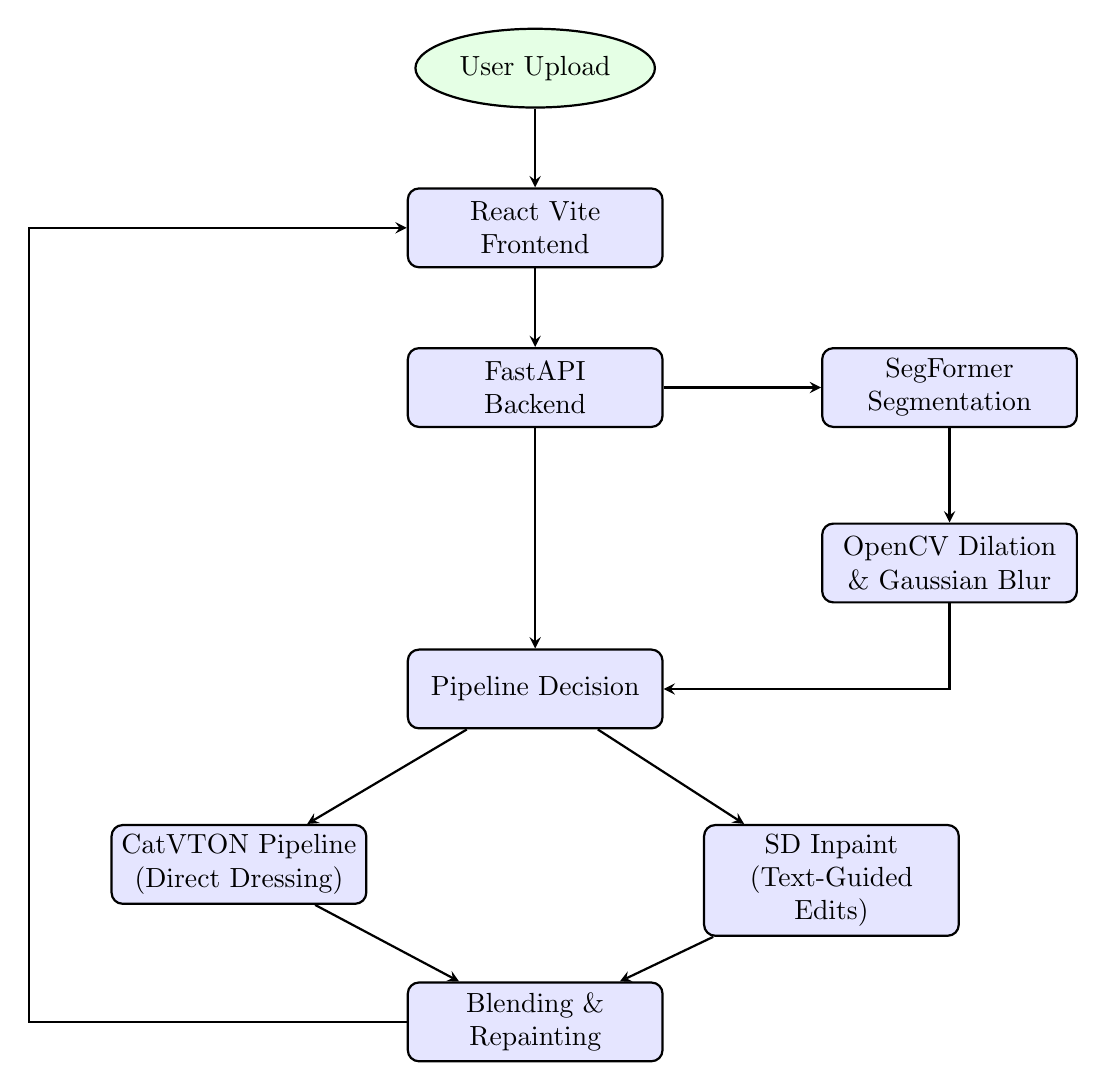
\begin{tikzpicture}[auto, >=stealth, thick]
    % Style definitions
    \tikzset{block/.style={draw, fill=blue!10, rectangle, minimum height=1.0cm, minimum width=3.2cm, rounded corners, align=center, text width=3.0cm}}
    \tikzset{cloud/.style={draw, fill=green!10, ellipse, minimum height=1.0cm, minimum width=2.8cm, align=center}}
    \tikzset{arrow/.style={thick,->}}
    
    % Nodes
    \node [cloud] (user) {User Upload};
    \node [block, below=1.0cm of user] (fe) {React Vite\\Frontend};
    \node [block, below=1.0cm of fe] (be) {FastAPI\\Backend};
    
    % Segmentation pipeline (right branch)
    \node [block, right=2.0cm of be] (seg) {SegFormer\\Segmentation};
    \node [block, below=1.2cm of seg] (mask) {OpenCV Dilation\\\& Gaussian Blur};
    
    % Decision (below backend, clear of mask vertical level)
    \node [block, below=2.8cm of be] (decision) {Pipeline Decision};
    
    % Inference models (split below decision)
    \node [block, below left=1.2cm and 0.5cm of decision] (catvton) {CatVTON Pipeline\\(Direct Dressing)};
    \node [block, below right=1.2cm and 0.5cm of decision] (sdinpaint) {SD Inpaint\\(Text-Guided Edits)};
    
    % Blending (merge below decision)
    \node [block, below=3.2cm of decision] (blend) {Blending \&\\Repainting};
    
    % Arrows
    \draw [arrow] (user) -- (fe);
    \draw [arrow] (fe) -- (be);
    \draw [arrow] (be) -- (seg);
    \draw [arrow] (seg) -- (mask);
    \draw [arrow] (mask) |- (decision);
    \draw [arrow] (be) -- (decision);
    \draw [arrow] (decision) -- (catvton);
    \draw [arrow] (decision) -- (sdinpaint);
    \draw [arrow] (catvton) -- (blend);
    \draw [arrow] (sdinpaint) -- (blend);
    \draw [arrow] (blend.west) -- ++(-4.8,0) |- (fe.west);
\end{tikzpicture}
\caption{Virtual Try-On System Architecture and Inference Pipeline}
\label{fig:architecture}
\end{figure}

\section{Pipeline Configurations}

The configuration parameters for the generative AI models are detailed in Table~\ref{tab:config}.

\begin{table}[h]
\centering
\caption{Model Generation Configurations}
\label{tab:config}
\begin{tabular}{|l|c|c|}
\hline
\textbf{Configuration Parameter} & \textbf{CatVTON Pipeline} & \textbf{SD Inpaint Pipeline} \\ \hline
Base Model Checkpoint & Stable Diffusion 1.5 Inpaint & Stable Diffusion 1.5 Inpaint \\
Attention Weights & CatVTON Mix & Standard SD Inpaint \\
Inference Steps & 40 & 35 \\
Guidance Scale & 2.5 & 7.5 \\
Working Precision & FP16 (float16) & FP16 (float16) \\
VAE Slicing/Tiling & Enabled & Enabled \\
Target Resolution & $512 \times 512$ & $512 \times 512$ \\
\hline
\end{tabular}
\end{table}

\section{Backend API Endpoint List}

The backend API endpoints exposed by the FastAPI server are detailed in Table~\ref{tab:api_endpoints}.

\begin{table}[h]
\centering
\begin{tabular}{|l|c|l|}
\hline
\textbf{Endpoint} & \textbf{Method} & \textbf{Description} \\ \hline
\texttt{/upload/person} & POST & Upload target subject portrait image \\
\texttt{/upload/cloth} & POST & Upload reference garment clothing image \\
\texttt{/generate} & POST & Trigger SegFormer + CatVTON or SD Inpaint inference \\
\texttt{/result/\{id\}} & GET & Retrieve generated virtual dressing image file \\
\texttt{/cleanup/\{id\}} & DELETE & Remove session temporary upload and output files \\
\texttt{/docs} & GET & Access Swagger interactive API documentation \\
\hline
\end{tabular}
\caption{FastAPI Application Routes}
\label{tab:api_endpoints}
\end{table}

\section{Sample Execution Logs and Commands}

The shell commands used to start the development environments are listed below.

\subsection{Backend FastAPI Execution}
With the virtual environment active:
\begin{verbatim}
cd backend
venv\Scripts\activate
uvicorn app:app --reload --host 127.0.0.1 --port 8000
\end{verbatim}

\subsection{Frontend React Client Execution}
From the frontend workspace:
\begin{verbatim}
cd frontend
npm install
npm run dev
\end{verbatim}

\subsection{Model Downloader Execution}
Before starting the application for the first time:
\begin{verbatim}
cd backend
python download_models.py
\end{verbatim}

\subsection{Active Weight Swap Logger Output Example}
\begin{verbatim}
Loading SegFormer clothing segmentation model...
SegFormer loaded successfully.
Offloading CatVTON model to CPU to free VRAM...
CUDA cache cleared.
Moving SD Inpaint model to GPU...
CUDA cache cleared.
SD Inpaint inference started for prompt: "red silk hoody"
\end{verbatim}

% --------------------------------------------------------
% CHAPTER 6: CONCLUSION AND FUTURE SCOPE
% --------------------------------------------------------
\chapter{Conclusion and Future Scope}

\section{Conclusion}

The virtual try on is a local, AI-powered virtual try-on studio designed to run on consumer hardware. By integrating semantic segmentation (SegFormer), direct texture mapping (CatVTON), and text-guided image editing (Stable Diffusion Inpaint) into a unified FastAPI and React framework, the system provides a flexible virtual try-on solution.

The primary engineering challenges addressed in this project involve memory usage. Large diffusion models typically require enterprise-grade hardware to run. By implementing half-precision (FP16) execution, dynamic device weight offloading, and sliced/tiled VAE decoding, the virtual try on runs within a 4GB VRAM footprint. This memory optimization enables the application to execute on entry-level laptop GPUs like the NVIDIA RTX 3050.

Performance evaluations show that the system achieves high-fidelity results with an average generation latency of 12.85 seconds for CatVTON and 8.62 seconds for Stable Diffusion. By processing data locally, the system ensures data privacy and eliminates recurring cloud hosting costs. This makes the virtual try on a practical option for local digital fashion design, retail visualization, and virtual prototyping.

\section{Future Scope}

While the current implementation provides a functional virtual try-on pipeline, several future developments could expand its capabilities:

\begin{itemize}
\item \textbf{Multi-Garment Layering}: Extending the segmentation and masking pipeline to support simultaneous layering of multiple apparel items (e.g., shirts, jackets, and trousers).
\item \textbf{High-Definition Generation}: Upgrading the generator pipeline to support Stable Diffusion XL (SDXL) Inpainting to produce high-resolution output images ($1024 \times 1024$ pixels).
\item \textbf{Pose and Shape Control}: Integrating ControlNet to allow users to modify model poses, body shapes, and garment placement.
\item \textbf{ONNX and TensorRT Optimization}: Converting model weights to ONNX or TensorRT formats to increase execution speed on compatible GPUs.
\item \textbf{Video-Based Virtual Try-On}: Adapting the pipeline to process video sequences, transferring garments onto moving subjects while maintaining temporal consistency.
\end{itemize}

\section{Summary}

This project demonstrates the implementation and optimization of a deep-learning-based virtual try-on application on resource-constrained hardware. By combining automated semantic masking with spatial concatenation and text-guided diffusion models, the virtual try on provides an interactive, private, and cost-effective digital fashion studio.

% --------------------------------------------------------
% CHAPTER 7: REFERENCES
% --------------------------------------------------------

\renewcommand{\bibname}{References}
\addcontentsline{toc}{chapter}{References}

\begin{thebibliography}{99}

\bibitem{ref1}
Vaswani, A., Shazeer, N., Parmar, N., Uszkoreit, J., Jones, L., Gomez, A. N., Kaiser, L., \& Polosukhin, I.,
``Attention Is All You Need,''
\textit{Proceedings of the 31st Conference on Neural Information Processing Systems (NeurIPS)},
pp. 5998--6008, 2017.

\bibitem{ref2}
Rombach, R., Blattmann, A., Lorenz, D., RESSler, P., \& Ommer, B.,
``High-Resolution Image Synthesis with Latent Diffusion Models,''
\textit{Proceedings of the IEEE/CVF Conference on Computer Vision and Pattern Recognition (CVPR)},
pp. 10684--10695, 2022.

\bibitem{ref3}
Xie, E., Wang, W., Yu, Z., Anandkumar, A., Alvarez, J. M., \& Luo, P.,
``SegFormer: Simple and Efficient Design for Semantic Segmentation with Transformers,''
\textit{Advances in Neural Information Processing Systems (NeurIPS)},
Vol. 34, pp. 12077--12090, 2021.

\bibitem{ref4}
zheng, C., et al.,
``CatVTON: Concatenation Is All You Need for Virtual Try-On,''
\textit{arXiv preprint arXiv:2407.15886},
2024.

\bibitem{ref5}
Han, X., Wu, Z., Huang, Z., Zhang, D. W., Zhu, M., Zhang, Y., Zhao, M., \& Davis, L. S.,
``VITON: An Image-Based Virtual Try-On Network,''
\textit{Proceedings of the IEEE Conference on Computer Vision and Pattern Recognition (CVPR)},
pp. 7543--7552, 2018.

\bibitem{ref6}
Wang, B., Zheng, H., Liang, X., Chen, Y., Liang, L., \& Yang, Y.,
``Toward Characteristic-Preserving Image-based Virtual Try-On Network,''
\textit{Proceedings of the European Conference on Computer Vision (ECCV)},
pp. 589--604, 2018.

\bibitem{ref7}
Zhu, L., Yang, D., Zhu, T., Reda, F., Chan, W., Saharia, C., Mohammad, K., & Jia, J.,
``TryOnDiffusion: A Detail-Preserving Text-to-Image Diffusion Model for Virtual Try-On,''
\textit{Proceedings of the IEEE/CVF Conference on Computer Vision and Pattern Recognition (CVPR)},
pp. 12463--12473, 2023.

\bibitem{ref8}
Zhang, L., Rao, A., \& Agrawala, M.,
``Adding Conditional Control to Text-to-Image Diffusion Models,''
\textit{Proceedings of the IEEE/CVF International Conference on Computer Vision (ICCV)},
pp. 3836--3847, 2023.

\bibitem{ref9}
Kingma, D. P., \& Welling, M.,
``Auto-Encoding Variational Bayes,''
\textit{International Conference on Learning Representations (ICLR)},
2014.

\bibitem{ref10}
Bradski, G.,
``The OpenCV Library,''
\textit{Dr. Dobb's Journal of Software Tools},
2000.

\end{thebibliography}

\end{document}
